\chapter{Conception et développement}

	\section{Architecture du logiciel}

		\subsection{Vision globale}
			
			D'un point de vue matériel, le projet est séparé en deux parties: la plateforme mobile, robot sur lesquels sont connectés les périphériques de capture, et le poste de contrôle, terminal de consultation des informations par l'opérateur humain. Cette architecture simple se retrouve dans le schéma \todoref.
			\change[inline]{Ajouter schéma archi wifibot[camera,lidar,rpi] <-> poste contrôle[pc,hid,ecran]}
			\par
			La plateforme mobile est un \emph{WiFiBot Lab V3}\cite{wifibot}, fourni par l'INSA Centre-Val-de-Loire, dont la carte de contrôle, munie d'un processeur x86, fonctionne sous \emph{Windows XP Embedded} et dispose d'un serveur connecté par WiFi à un routeur (fourni également) permettant de lui envoyer des commandes de contrôle des moteurs des roues. Dans un souci de conservation de l'existant et par simplicité de développement, nous avons choisi de contrôler les périphériques et de centraliser les transfers de données au travers d'un \emph{Raspberry Pi 3b}, qui possède une puissance de calcul raisonnable face à sa faible consommation et une carte WiFi intégré. Par ailleurs, le fait que micro-ordinateur fonctionne sous \emph{Linux} nous permet de conserver une continuité dans le choix des technologies logicielles à utiliser.
			\par
			Le poste de contrôle, connecté au même routeur que le WifiBot, est constitué d'un micro-ordinateur disposant d'un \gls{gpu} dédié (NVIDIA K620), d'un écran et de périphériques d'entrées standard (clavier, souris), permettant d'intéragir avec l'opérateur. Au vu de la faible puissance de calcul dont dispose la plateforme mobile, le choix a été fait de centraliser les traitements lourds sur ce poste.
			\par
			Le logiciel se scinde en deux parties bien distinctes:
			\begin{description}[noitemsep]
				\item[l'Interface Homme-Machine], qui permet à l'opérateur de contrôler les mouvements de la plateforme mobile, démarrer les périphériques de capture et leurs chaînes de traitement, d'enregistrer une mission et de visionner le déroulement d'une mission enregistrée.
				\item[le réseau de traitement de données], qui permet d'exploiter les données en sortie des périphériques de capture de manière à en tirer des informations pertinentes: la cartographie des lieux visités et les objets d'intérêt qui y sont présents.
			\end{description}
			Cette architecture se retrouve en \todoref, avec des éléments détaillant le fonctionnement de chaque partie.
			\change[inline]{Ajouter schéma archi logiciel général}

		\subsection{Réseau de traitement de données}

			\change[inline]{Ajouter schéma réseau ros}
			\content[inline]{A faire}
			
		\subsection{Interface Homme-Machine}
		
			\change[inline]{Ajouter schéma archi ihm}
			\content[inline]{A faire}

	\section{Détails d'implémentation}
	
		\subsection{Transmission de la vidéo}
		
			La caméra Ricoh Theta S comporte une carte WiFi, ce qui permet, pour une utilisation \og normale \fg{} (avec l'application Android fournisseur) de s'y connecter avec un téléphone fonctionnant sous Android, afin d'y transférer les données de la caméra. Ces données peuvent prendre la forme de photos ou de vidéos, préalablement enregistrées sur la mémoire interne de la caméra et donc récupérées en différé, ou d'un mode spécial, nommé \emph{live}, qui permet de transmettre un flux vidéo continu correspondant à la capture des objectifs de la caméra en temps réel. Ce mode permet de transmettre un aperçu au téléphone avant de prendre une photo, uniquement supporté par l'application Android du fabricant. Devant la demande croissante du public d'utiliser ce mode de \og livestream \fg{}, les développeurs ont choisi de le rendre disponible sur pc, au travers d'un pilote matériel permettant aux OS \emph{Windows} et \emph{Mac OS} de considérer la caméra, alors branchée à l'ordinateur par \gls{usb}, comme une webcam, permettant ainsi la plupart des programmes d'exploiter ce flux vidéo. Ce pilote se charge de communiquer avec le bon protocole les commandes utilisateurs à la caméra et de transformer le flux vidéo dans un format exploitable. Après analyse du pilote windows, il a été découvert (car non exprimé dans la documentation du produit) qu'il utilise la bibliothèque \emph{libUVC}, et donc que la communication avec la caméra est effectuée au travers du protocole \gls{uvc}. La caméra étant sur la plateforme mobile disposant d'un \emph{Raspberry Pi 3b}, il a été développé un noeud \gls{ros} permettant de lui envoyer des commandes, d'acquérir le flux vidéo direct et de l'envoyer sur le poste de contrôle.
			\par
			Une problématique arrivée rapidement est celle de la transmission sur le WiFi.
			La Raspberry Pi dispose d'une carte WiFi qui ne supporte que la norme 802.11g, et ne peut donc transférer des données qu'au débit réel maximal de 25 Mb/s.
			Après une analyse de paquet en cas réel, la bande passante disponible pour le flux vidéo n'est que de 17,6 Mb/s, soit 2,2 Mo/s.
			Une image \gls{jpeg} en sortie de la caméra pèse en moyenne 400ko, et la caméra opère à 15 images/s, ce qui nécessite un débit de 6M/s.
			La Raspberri Pi dispose d'un \gls{gpu} \emph{VideoCore IV}\cite{videocore}, servant en priorité à encoder et décoder des vidéos (par exemple, pour lire un flux vidéo en haute qualité depuis internet).
			Il est donc possible d'utiliser la bibliothèque \emph{OpenMAX} pour encoder une vidéo, qui devrait donc peser moins qu'une séquence d'images décorrélées.
			Cependant, après de nombreux éssais d'envoi de flux converti (au format h264, le format le plus optimisé pour cette puce graphique), il s'est avéré que l'encodage entraîne un surplus de traitement au niveau du processeur de la Raspberry, qui entraîne l'introduction d'une latence importante entre la capture d'une image et sa visualisation sur le poste opérateur.
			Il a donc été décidé de réduire la vitesse du flux de la caméra à 5 images/s, afin de ne nécessiter que 2Mo/s de bande passante.
			%1 jpeg 1280x768 = 400ko
			% 5 fps = 2000ko/s
			%15 fps = 6000ko/s
			%wifi        54   mb/s | 6.75  mo/s
			%            25   mb/s | 3.125 mo/s
			%benchmarks: 17.6 mb/s | 2.2   mo/s
			\par
			Les images sont donc extraites des paquets \gls{usb} et envoyées au poste de contrôle encapsulées dans un protocole simple et efficace pour la transmission de données unidirectionnelle en temps réel, dont l'unité de donnée (\gls{pdu}) est la suivante:

			\begin{center}
				\scriptsize
				\begin{tabularx}{\textwidth}[h]{|Y|Y||Y|}
					\toprule
					\multicolumn{2}{|c||}{entête (24 octets)} & charge utile (variable) \\
					\midrule
					Identifiant protocole (8 octets) & taille image (16 octets) & données (variable)\\
					\bottomrule
				\end{tabularx}
			\end{center}

			Ces trames sont encapsulées dans des trames \gls{tcp} pour laisser le système s'occupper de la fragmentation et de l'ordonnacement, ce qui simplifie le traitement du côté réception et du côté traitement des données (pas de mise en file d'attente).
			
		\subsection{Transformation vidéo}
		\label{sub:transfo}
		
			En sortie de la caméra, l'image correspond aux photos prises par les deux objectifs, chacun ayant un angle de prise de vue de $190^{\circ}$, horizontalement et verticalement, et chacun étant de type \gls{fisheye} circulaire. Un exemple d'image non traitée est représenté \autoref{fig:rawcapture}. Le fait de disposer de deux photos \gls{fisheye} qui couvrent l'ensemble du point de vue à la position de la caméra s'appelle couramment \emph{Dual Fisheye}. On peut parler de représentation sphérique d'un point de vue, l'angle de champ étant de $360^{\circ}\times180^{\circ}$. Les caractéristiques spatiales visibles observent un niveau de déformation proportionnel à leur éloignement du centre de l'objectif. À défaut de traitement, la détection et la classification des objects contenus dans la scène présentent des imprécisions qui rendent de tels résultats inexploitables.
			\begin{figure}[h]
			{
				\centering
				\includegraphics[width=1\textwidth]{figures/capture.jpg}
				\caption{Image non traitée capturée en sortie de la caméra}
				\label{fig:rawcapture}
			}
			\end{figure}
			\par
			Comme évoqué dans la section précédente, le pilote fourni par le fabricant transforme cette image en appliquant une projection spatiale sur chacun de ses pixels de manière à obtenir une couverture complète du point de vue en projection équirectangulaire. Cette méthode permet de voir l'intégralité de la surface d'une sphère sur un plan. Les figures suivantes visent à illustrer cette opération.
			On considère la scène \autoref{fig:cage}, où notre point de vue correspond à la sphère rouge. Notre scène comporte donc une cage dont les faces ont des couleurs différentes et des numéros permettant de mettre les caractéristiques spatiales en valeur.
			\begin{figure}[h]
			{
				\centering
				\includegraphics[width=0.6\textwidth]{figures/cage.png}
				\caption{Scène d'exemple vue de l'extérieur}
				\label{fig:cage}
			}
			\end{figure}
			\par
			On se place maintenant à l'intérieur, en direction du côté violet (face du fond), et on prend deux photographies -- respectivement vers l'avant et vers l'arrière -- à l'aide d'un objectif \gls{fisheye} avec un angle de champ de $180^{\circ}$. On obtient alors l'ensemble du point de vue sous la forme de deux disques comme vus en \autoref{fig:dualfish}.
			\begin{figure}[H]
			{
				\centering
				\includegraphics[width=1\textwidth]{figures/dfish.png}
				\caption{Vue sphérique \og dual fisheye \fg{}}
				\label{fig:dualfish}
			}
			\end{figure}
			\par
			On crée alors un rectangle où chaque pixel trouve un correspondant dans ces disques, et on obtient une projection equirectangulaire de l'espace sphérique d'origine. (\autoref{fig:equirect}).
			\begin{figure}[H]
			{
				\centering
				\includegraphics[width=1\textwidth]{figures/equirect.png}
				\caption{Projection equirectangulaire}
				\label{fig:equirect}
			}
			\end{figure}
			L'opération mathématique revient à effectuer trois projections spatiales successives pour chaque pixel, ce qui justifie l'emploi d'un processeur graphique (haute parallélisation des calculs).
			\par
			La première projection revient à retrouver les coordonnées sphériques réelles de l'objectif de la caméra à partir des coordonnées polaires des disques \emph{fisheye}. En effet, l'objectif est vu comme une hémisphère imparfaite (base circulaire mais profondeur moindre), dont la profondeur est représentée par la distance focale $f$.
			\begin{figure}[htb]
				\centering
				\begin{minipage}{.5\textwidth}
					\centering
					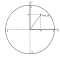
\includegraphics[width=0.95\linewidth]{figures/polar.pdf}
					\captionof{figure}{Coordonnées cartésiennes sur image fisheye}
					\label{fig:pcart1}
				\end{minipage}%
				\begin{minipage}{.5\textwidth}
					\centering
					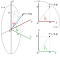
\includegraphics[width=0.95\linewidth]{figures/spherical.pdf}
					\captionof{figure}{Coordonnées sphériques}
					\label{fig:def1}
				\end{minipage}
			\end{figure}

			
			Bien qu'elles soient toujours déformées, les faces orange et verte deviennent assez linéaires pour présenter des caractéristiques spatiales détectables. On opère alors la détection sur cette image.

		\info[inline]{WIP}

		\subsection{Détection et Classification}
		
			\lipsum[5]
			\content[inline]{A faire}
			
		\subsection{Présentation vidéo et incrustation}
		
		\begin{figure}[htb]
			\centering
			\begin{minipage}{.5\textwidth}
				\centering
				\includegraphics[width=0.95\linewidth]{figures/def0.png}
				\captionof{figure}{Image equirectangulaire}
				\label{fig:def0}
			\end{minipage}%
			\begin{minipage}{.5\textwidth}
				\centering
				\includegraphics[width=0.95\linewidth]{figures/def1.png}
				\captionof{figure}{Texture mapping }
				\label{fig:def1}
			\end{minipage}
			
			\vspace{0.5cm}
			
			\begin{minipage}{.5\textwidth}
				\centering
				\includegraphics[width=0.95\linewidth]{figures/def2.png}
				\captionof{figure}{Déformation}
				\label{fig:def2}
			\end{minipage}%
			\begin{minipage}{.5\textwidth}
				\centering
				\includegraphics[width=0.95\linewidth]{figures/def3.png}
				\captionof{figure}{\emph{Sphere mapping}}
				\label{fig:def3}
			\end{minipage}
		\end{figure}
		\content[inline]{A faire}
			
		\subsection{Contrôle du robot}
		
			\lipsum[1]
			\content[inline]{A faire}
			
		\subsection{Modularité de l'IHM}
		
			\lipsum[2]
			\content[inline]{A faire}
			
	\section{Méthodes de travail}

		\subsection{Git-flow}
		
			\lipsum[3]
			\content[inline]{A faire}
			
		\subsection{Emprunts agiles}
		
			\lipsum[4]
			\content[inline]{A faire}
			

	\section{Pérennisation du projet}
	
		\subsection{Manuel utilisateur}
		
			Le projet est destiné à être poursuivi lors de stages ultérieurs, c'est pourquoi il a été décidé de rédiger un manuel d'utilisation, autant à l'intention des développeurs que pour un utilisateur \og opérateur \fg{}. Il regroupe un manuel d'installation, un guide de résolution des problèmes, un manuel d'utilisation de l'interface homme-machine et un guide de développement, qui explique le fonctionnement du logiciel et propose des améliorations possibles.
			\par
			Ce manuel a été rédigé en Markdown \cite{markdown}, un langage de balisage léger permettant une mise en forme rapide du texte et l'inclusion d'images. Il est compilé sous la forme d'un site html statique par MkDocs\cite{mkdocs}, ce qui permet une mise en forme agréable, ainsi qu'une navigation simple et plus intuitive qu'un document \og classique \fg{}. Il est donc prêt à être hébergé sur un serveur web.
			
		\subsection{Documentation}
		
			\content[inline]{A faire}
			
		\subsection{Installation automatique}
		
			\content[inline]{A faire}
				
		\subsection{Communication interne}
		
			\content[inline]{A faire}
